\hypertarget{software-architectures}{%
\section{Software Architectures}\label{software-architectures}}

Consider a typical robot or the architecture of the mobile robot
described in ~\texttt{fig:intro-components}. There is only one computer
involved in the sample system. How could distributed computing be part
of the equation? It is plausible that parallel computing could be
involved, but at first blush we might suppose that this would be a
multi-core issue which is managed by the operating system. So again, why
would distributed systems be of interest?

At a very low level, we have basic sensor hardware, motor and servo
hardware and communications hardware. These live in a real time world
and have dedicated hardware. These are embedded devices which can then
communicate with the main system through standard interfaces such as USB
or i2c. Each one runs at different frequencies with different control
systems. It is interesting to watch the development of current robot
infrastructures. In some ways it wants to follow the path the
traditional operating systems did over the last 50 years. In other ways
this development benefits from the last half century.

Think for a moment about traditional program design and execution. The
process lives in an address space which is defined as all of the memory
addresses for which the program resides and
accesses,~\texttt{fig:address\_space}.

\begin{quote}
Address space for a process.
\end{quote}

The underlying operating system will go to great lengths to contain the
process in it's allocated section of memory. Separate processes are run
in separate contexts where the hardware isolates the code. In addition
to the address space, processes no longer share registers, stack, files,
etc. The OS does this to protect code blocks from each other. Errors in
one system do not corrupt other systems (such as a faulty end condition
on a loop writing to memory). Unintended interactions are greatly
reduced. This is the design philosophy of any modern operating system.
The OS manages the resources and provides the programs the illusion that
they live alone on the computer. Each program runs as if it owns the
entire machine. It appears to the program that it gets the entire memory
system, disk system and networking. The OS does all the heavy lifting.

The other thing the OS is doing is giving the program a common interface
to the hardware below. Meaning that the program (well, the programmer)
need not worry about if the storage device is from vendor A or B. You
don't need to know anything about the device specifics. There are
general interfaces for the memory system, file system, devices, etc.
This provides portability with software and really reduces the
programming effort. So the OS provides the illusion of an abstracted
computer or a virtual computer~\texttt{fig:os-abstract}.

\begin{quote}
The fundamental machine abstraction.
\end{quote}

The common interface is implemented by a series of system calls. These
are very special functions which allow access to the hardware. They are
not traditional function calls since the thread of execution is moved
over to the operating system. The kernel manages access and permissions,
performs the requested function or returns error codes, and the process
execution resumes. A current OS attempts to provide an abstract machine
for a process. Low level OS routines (drivers and modules) are expected
to translate the specifics of talking to a particular piece of hardware
to the general abstracted interface. This means the programmer just
interacts with a generic storage device and is not concerned about the
specific details of that device. Actually, the interface makes one not
even worry about the type of technology, for example magnetic vs solid
state. This same approach is needed in the robotics world. The USB
interface has helped with modular hardware in a limited sense. This
makes the development and maintenance of software much easier. It also
makes the system much more secure and robust. Being able to program
using a fixed set of system calls makes the developer's job easier which
in turn reduces errors. It means that the tricky part of accessing the
hardware is done by individuals experienced in that domain. The
collection of system calls really defines the OS. Not so much the
collection of software shipped or the choice of desktop GUI.

It begs the question, if the operating system is really designed to
separate processes, then how do they communicate. Processes must have
communication. So various types of interprocess communication have been
devised to support the model of breaking computation into multiple
execution contexts, but still providing a way for the processes to
communicate and coordinate.

For the moment, assume you are going to write your robot control code.
Your code is a large sequence of sensing, planning and moving. The
planning code probably runs on the CPU and at megahertz speeds. The
sensing at kilohertz speeds and the movement at hertz speeds. As
mentioned above you have lots of different activities at different
speeds. We should take a page from the CS history books. We need modular
code. We need code that is interrupt driven. We need to separate the
different components.

Just like with desktop processing, it is neither possible or desirable
to place all of the code into a single address space running on a single
event loop. Even if we could place all of the sensor/actuator driver
routines into the same program, good design demands modular code. It is
essential to break the software into components. Separate them. This is
done for ease of design, maintenance, security, robustness, and fault
tolerance. At times you don't even have a choice about modularity. The
current state of robotics development is that no single vendor builds
all of the parts for the robot. You must assemble the hardware from
different systems. The drivers for the components are provided. Robotics
systems are too large to write from scratch. They live on top of
existing traditional computing devices. What does this mean?

The first thing we want to address is the separation of data. This is
often approached by data encapsulation approaches found in object
oriented programming. Robotics has grown out of an embedded world
focused on controls. These were real time systems with hard constraints
on response times. By design the real time operating system and the
underlying hardware was not running full operating systems on high
performance computing hardware. So object oriented programming may not
have been viable due to lack of system support. However, now one can get
very powerful machines and full featured operating systems on postage
stamp sized systems. OOP provides ways to limit access of data and deal
with the complexities of large code installations.

We also want to separate the different functional blocks into different
execution blocks. Again OOP support can support the programmer in moving
to concurrent execution of methods. At a lower level, concurrency is
supported by the notion of threads. A thread is an execution context.
This means that the thread has a program counter, registers and a stack,
but may share the address space which contains the data. Multithreaded
programming gives the developer concurrency, but possibly at great cost.
Some of the most subtle and difficult errors can arise when multiple
threads are working on a common data block. Constructs such as
semaphores have been created to manage access to common data regions.
However, semaphores can cause deadlocking or process starvation.

Experience in both OOP and shared memory programming is important to
avoid disastrous results. Another issue is the pace of robotics
software. Systems have become increasing complicated over time.
Expertise in all areas is hard to find. The ability to use external
routines for certain aspects of the system - especially in development
is critical. Having a large collection of functionally distinct modules
makes the software akin to the building blocks found in hardware. Just
as hardware systems are separate but use common interfaces (such as
common pinouts in Arduino, or interfaces such as USB), software systems
need to do the same thing to realize their potential.

Programs then must communicate with other programs using standard
communication channels. One approach is to build each program as a
function in a library or a class. Pushing code into a library can be a
software engineering trap. Development is challenging enough when you
have a huge interconnected codebase and then add hardware uncertainty.
There are a thousand variations to a robot due to the number of sensors,
actuators, and software libraries. One does not want to rebuild the
system each time an update is released. A class will help with
encapsulation. Still, this metaphor is one of single address space
programming (yes, threads can help). Shared memory has been a favorite
due to it's speed. Even so, it is fraught with danger. A course in
operating systems shows you how shared memory programming can lead to
problems far worse than low performance with the ability to completely
deadlock a system. Another issue is that there are probably multiple
processing units involved which don't share memory and so threaded
models do not apply.

Multithreaded computation or shared memory programming is not the only
way to proceed. Another form of interprocess communication is known as
message passing. Data and computation requests are actively managed.
Data is packaged and sent off to remote processes; processes which do
not share the address space. These processes can be on different
machines with different operating systems. This is increasingly
important since the sensors and controllers are requiring their own
cpus. Message passing is a way to address the interprocess communication
need and also support multiple CPUs which do not share memory.

To support message passing interprocess communication, we need a way to
send a packet of data to a remote host. The Unix world developed sockets
as a method to send packaged data. Sockets and their supporting
infrastructure are the backbone of the internet. Network sockets are the
foundation of the internet which is probably the largest distributed
system on the planet. Using message passing interprocess communication
built over network sockets, we can build our collaborating process
groups. Sockets allow us to define a standard interface for
communication and then indirectly for computation. Building our software
components on a message passing architecture built on TCP/IP simplifies
the software engineering process. It embraces the robot as a distributed
system from the start. Asynchronous concurrent computing can proceed in
this environment. Scaling the number of devices is easier. Moving to
swarms of robots and having them act as a single system is a natural
outgrowth.

Robotics software followed some of the development seen in the general
computing world. Microcontrollers without an operating system running
programs resident in a single memory space. Adding functions, hardware
and external devices pushed for having more complicated operating system
support. Real time operating systems and desktop operating systems found
their way into robot hardware. As more demands on motion planning
occurred, increasingly powerful machines entered. This was made possible
by the increasing power and shrinking size of the cpu.

Operating Systems development saw large monolithic kernels like
unix,~\texttt{fig:os-monolithic}. They were powerful, provided
sufficient performance and were complicated. Protection of resources and
program portability became common. A complicated system call interface
was produced to support the separation of user program from hardware.
However, difficulties in development and debugging lead to layered OS
designs such as early NT and OS/2,~\texttt{fig:os-layered}.

\begin{quote}
Monolithic

Layered
\end{quote}

Separation of code blocks is not complete in either of the previous
designs and so experiments to build a minimal kernel, one which used
message passing to support interprocess communication, was created.
These were known as microkernels since the design promoted moving all
but the bare minimum out of the kernel leaving a very small kernel code
base.

\begin{quote}
Microkernel architecture.
\end{quote}

The concept of a micro-kernel is very appealing. So much so that the
Mach and NT kernels adopted the approach. The downfall was performance.
As we embark on robotics development we cannot forget past experience.
Performance drove many systems back to a monolithic design. Certainly
the real time systems that run the hardware need real time code. Linux
and Solaris decided against a microkernel approach and went with
loadable modules. For an operating system, performance or speed is
critical.

So, should we follow the OS path? Is the situation the same? There are
two important differences in robotics. First is the domain of operation
and the second is the measure of performance. The domain for a robot is
the physical world. Mechanical systems operate in the millisecond range.
The gigahertz range is well beyond what can be expected from mechatronic
systems. Any code that interacts with the mechatronic system does not
take the performance hit like what is seen with CPU process groups and
so the benefits of this design stand out. The other aspect is the
measure of performance. Once the processor can respond in time for a
request, speeding it up may have no impact on the operation. Our measure
now turns to the effectiveness of the robot in the task, development
ease, security issues, cost, etc. So, again, we can see the benefit of
message passing architectures.

However, processing sensor data or the planning operations could require
considerable resources and partitioning the code into separate processes
must be done with care. A careful study of data flow and data
dependencies is required. This allows one to exploit available
concurrency. Then the design decisions can be made regarding how to
handle selection of the hardware and the resulting interprocess
communication.

Computer vision can lead to massive amounts of concurrent simple
arithmetic operations. A CPU may not be the best choice. Not that it
cannot be done since most of the time it is. However, we know that
specialized hardware can vastly outperform CPUs when confronted with
structured operations. Use of FPGAs and GPUs are two great examples of
different architectures that have been applied. This type of asymmetric
computing can greatly enhance the performance of a robot which is
simultaneously running vision, navigation and mapping. A system that is
able to distribute different types of computation over asymmetric
processors is now entering the distributed computing realm.

Consider a couple of applications of robotics. One is teleoperation and
another is telepresence (arguably related, but are good examples). One
of the driving forces in robotics is to remove people from dangerous and
harmful situations. To this end, we require that the user is some
distance away. Both applications require local and remote processing,
and both require very robust communication.

A generalized communication system is needed. Something that provides
uniform interfaces and is not dependent on specific hardware; a system
that allows for modules to reside in separate address spaces and even
separate processing units connected over a LAN. This system must be able
to operate in an asynchronous fashion and be tolerant of faults (such as
restarting a module).

\hypertarget{distributed-computation-and-communications}{%
\subsection{Distributed Computation and
Communications}\label{distributed-computation-and-communications}}

Robotics is evolving from having completely integrated monolithic
control systems to modular distributed architectures. As the hardware
becomes more powerful and the goals more sophisticated, the complexity
of the control system increases. It is increasing in a superlinear
manner. We may view the workings of robotics software as a collection of
interconnected computations and thus view the collection in a graph.
Nodes would represent computational blocks, specifically processes.
Interprocess communication is represented by the edges connecting the
nodes in the graph. The connection between two nodes is the point to
point communication we discussed above. A single robot could have many
nodes. Some that control low level aspects like drive motors or wheel
encoder data. Others higher level like processing data for computer
vision algorithms, estimating position or routing the robot over the
landscape.

Many of the nodes will be producing data for other nodes. Some nodes are
producers, some consumers and some are both. The underlying client
server architecture appears to be required. For a particular node that
produces data for several other nodes, it needs to be a server to those
client nodes. With multiple servers running and each delivering a
different service, how should we manage this? The system connects to a
host:port combination. So, one would need to know the host:port pair
apriori. The host name might be known, but what about ports? A system
could have external software that uses any particular port range. Having
the vast collection of sensors and user contributed computational nodes
means that a port numbering and classification system needs to be
devised. Unix systems used to have remote procedures bound to port
numbers. This works when there is a limited list. When the list gets
long we need something like the Dewey Decimal system in the library. Of
course we know that as the scale of node types increases, the
predetermined mapping will eventually break.

\begin{figure}
\centering
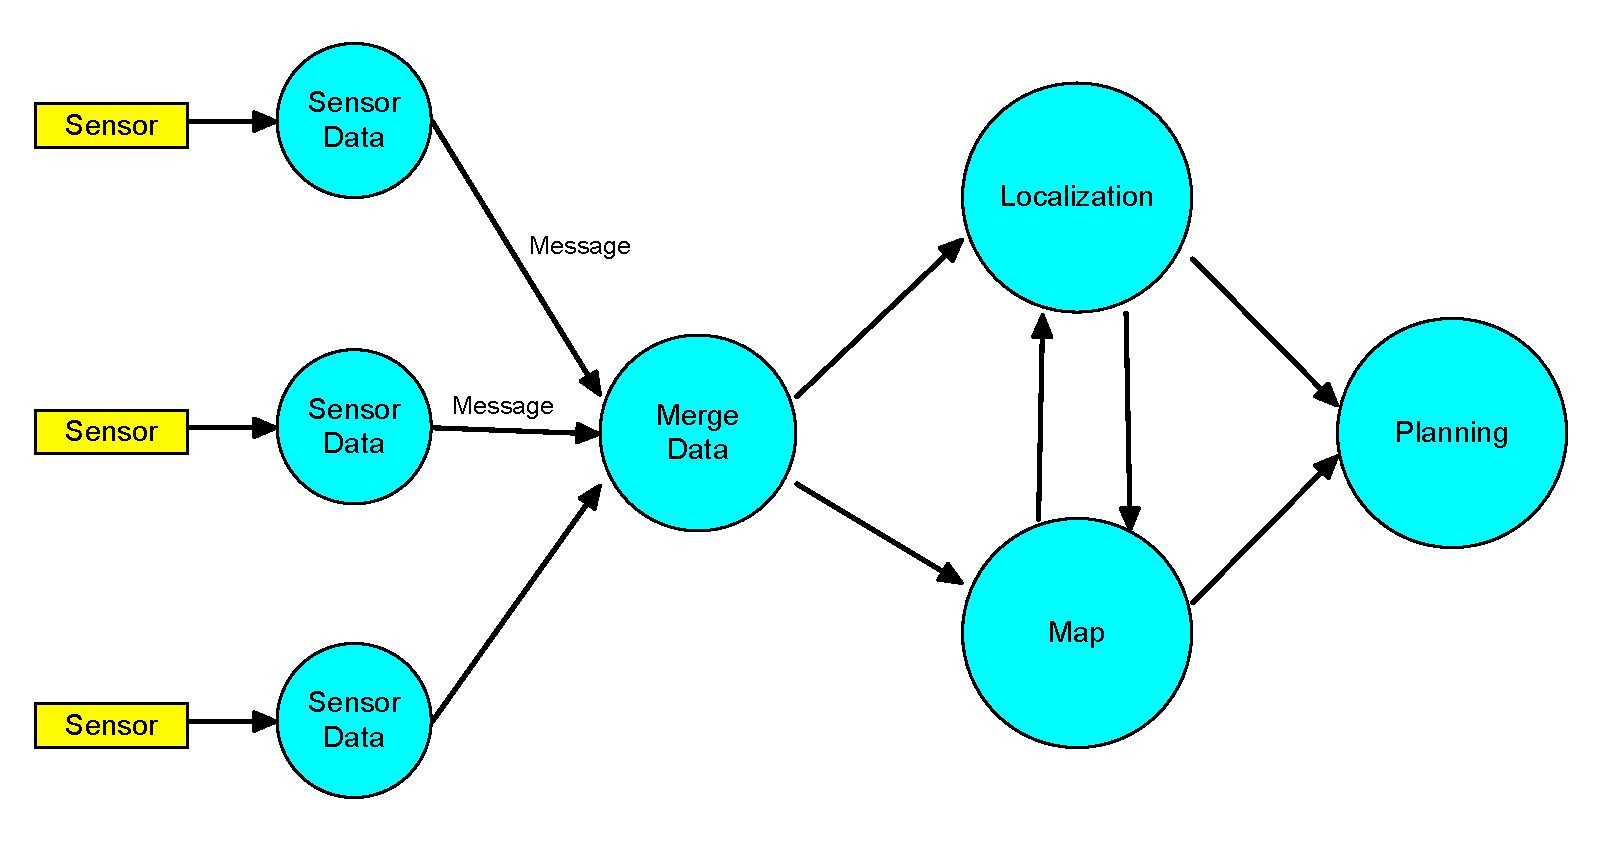
\includegraphics[width=0.9\textwidth,height=\textheight]{ToolsFigures/distrcomp.*}
\caption{}
\end{figure}

For small and medium sized systems, one can manage the communciations
using a central server. This works well in a variety of systems. For
larger systems, where hundreds or thousands of nodes appear in the
computation/communication graph, this produces a significant bottleneck
and will not scale at all. And so a centralized system will not work.
The system needs to be dynamic and configurable. However, we need a way
to allow the data producer to connect with the data consumer.

A peer to peer connection is desired to avoid bottlenecks and other
network issues related to a single central server. We also need a way to
dynamically map hosts and ports as the system needs. This means that a
database is required. The information can be centralized or distributed.
If scale allows, a centralized system will have better response bounds
since we know exactly how long it will take to find the required data. A
distributed database may require several requests to get the
information.

When a service starts up, it should register itself in a publicly
available database. It would register with a central server and record
that a particular service may be found at host:port pair. When the
client is ready, it can query the central repository, request the
service location and then connect to the correct server. This main
server or master is a nameserver. Having only the job of handing out
names at the start of the service, it does not affect the communications
later on. We will say a particular node with data ( the service) will
publish this data. This means that it registers with the name server and
accepts connections. A client requiring the data will subscript to the
data by requested the publishing node from the nameserver and then
requesting a connection to that node.

Having a specific service with multiple clients can complicate matters.
The point of the service is to produce something, not worry about
communications. So, to address this, a publish-subscribe mechanism can
be built that treats the data as a topic. That topic is available on a
type of message bus. The publisher and subscriber should be separated
and not know about each other. This way one can deal with issues of
scale, broken connections, reconnections and other real world issues
without disturbing either the publisher or subscriber. Of course this
will eliminate request-reply types of communication which should be
addressed using a direct point to point type of channel.

The communication systems discussed above are normally implemented using
a one of the standard Interprocess Communication interfaces. For this
text, will focus on Sockets. \texttt{Sockets} provide a bidirectional
channel between two processes. Although one side is setup like a server
and one side like a client, this is basically point to point type of
communication. With only two processes one could call this peer to peer
or client server, however, in this case it is strictly one process to
one process. The socket mechanism underneath is used to implement a vast
array of process to process communication methods. We will not program
sockets directly or natively, but will do this through a communication
library known as ZeroMQ. ZeroMQ is introduced in the next section.
